\section{Extensive Form Games}{\label{sec:efg}}
We have already seen the formal definition of Extensive Form Games (\ref{def:efg}).
The extensive form representation of a game provides a detailed and richly structured way to describe a game.
Specifically it captures:
\begin{itemize}
	\item who makes a move at any given time
	\item what actions each player may play
	\item what the players know before playing at each stage
	\item what the outcomes are as a function of the actions, and
	\item payoffs that players obtain from each outcome.
\end{itemize}
Extensive form games with a finite number of players and with a finite number of actions available to each player are depicted graphically using game trees.

In the game tree representation, the nodes are of three types:
\begin{itemize}
	\item root node (initial decision node)
	\item internal nodes (which are decision nodes)
	\item leaf nodes or terminal nodes (which are outcome nodes)
\end{itemize}
Each possible sequence of events that could occur in the game is captured by a path of links from the root node to one of the terminal nodes. When the game is played, the path that represents the sequence of events is called the \textbf{path of play}.
Each decision node is labeled with the player who takes a decision at that node.
Each decision node can be uniquely identified by a sequence of actions leading to that decision node from the root node.
Each node represents not only the current position in the game but also how it was reached.
The terminal nodes are labeled with the payoffs that the players would get in the outcomes corresponding to those nodes.

\subsection{Transforming Extensive Form to Strategic Form}
An extensive form game can be transformed into an equivalent strategic form game using the notion of a strategy.

$\mathbb{I}_i$ denotes the set of all information sets of player $i$ in the given game.
Let $A_i$ as usual denote the actions available to player $i$.
Given an information set $J \in \mathbb{I}_i$, let $C(J) \subseteq A_i$ be the set of all actions possible to player $i$ in the information set $J$. Then,
\begin{defn}[Strategy]
	A strategy $s_i$ of player $i$ is a mapping $s_i : \mathbb{I}_i \rightarrow A_i$ such that $s_i(J) \in C(J)\ \forall J \in I_i$.
\end{defn}
Shorthands for strategy profile
\begin{itemize}
	\item The index $-i$ is used to refer to all the players other than player $i$
	\item $s_{-i}$ is the strategy profile of all players other than player $i$
	\item Now, the complete strategy profile can be denoted as $(s_i, s_{-i})$
\end{itemize}
\begin{defn}[Outcome]
Given an extensive form game $\Gamma$ and a strategy profile $s = (s_1,\ldots,s_n)$ in the game, the outcome resulting out of the terminal history corresponding to the strategy profile $s$ is called the outcome of $s$ and is denoted by $O(s)$.
\end{defn}
\begin{note}
	Every extensive form game has a unique strategic form representation. The uniqueness is up to renaming or renumbering of strategies. We can also immediately observe that a given strategic form game may correspond to multiple extensive form games.
\end{note}
The strategy $s_i$ for player $i$ is a complete contingent plan that specifies an action for every information set of the player.
Let's dive into some examples.
\begin{exm}[Matching Pennies with Observation]{\label{exm:mp}}
	There are two players, 1 and 2, each of whom has a rupee coin.
	One of the players puts down his rupee coin heads or tails up.
	The other player sees the outcome and puts down her coin heads up or tails up.
	If both the coins show heads or both the coins show tails, player 2 gives one rupee to player 1.
	If one of the coins shows heads and the other coin shows tails player 1 gives one rupee to player 2.

	Depending on whether player 1 or player 2 moves first, there are two versions of this game. Figure \ref{fig:mpwo1} shows the game tree when player 1 moves first while Figure \ref{fig:mpwo2} shows the game tree when player 2 moves first.
	\begin{figure}[H]
		\centering
		\begin{subfigure}{0.45\linewidth}
		        \centering
		        \begin{tikzpicture}[scale=0.12, every node/.style={scale=0.7}]
		            \tikzstyle{every node}+=[inner sep=0pt]
		                \draw [black] (0,30) circle (2.5);
		                \draw (0,30) node {$1$};
		                \draw [black] (-15,15) circle (2.5);
		                \draw (-15,15) node {$2$};
		                \draw [black] (15,15) circle (2.5);
		                \draw (15,15) node {$2$};;
		                \draw (-25,-1) node {$(1,-1)$};
		                \draw (-5,-1) node {$(-1,1)$};
		                \draw (5,-1) node {$(-1,1)$};
		                \draw (25,-1) node {$(1,-1)$};
		                \draw (-8.5,23.5) node [left] {$H$};
		                \draw (8.5,23.5) node [right] {$T$};
		                \draw (-22,8) node [left] {$H$};
		                \draw (-8,8) node [right] {$T$};
		                \draw (8,8) node [left] {$H$};
		                \draw (22,8) node [right] {$T$};
		                \path [line] (-1.5,28) -- (-13,17.5);
		                \path [line] (1.5,28) -- (13,17.5);
		                \path [line] (-16.5,13) -- (-25,1);
		                \path [line] (-13.5,13) -- (-5,1);
		                \path [line] (13.5,13) -- (5,1);
		                \path [line] (16.5,13) -- (25,1);
		            \end{tikzpicture}
		            \caption{Player 1 moves first}
		            \label{fig:mpwo1}
		    \end{subfigure}
		    \vLine
		    \begin{subfigure}{0.45\linewidth}
		        \centering
		        \begin{tikzpicture}[scale=0.12, every node/.style={scale=0.7}]
		            \tikzstyle{every node}+=[inner sep=0pt]
		                \draw [black] (0,30) circle (2.5);
		                \draw (0,30) node {$2$};
		                \draw [black] (-15,15) circle (2.5);
		                \draw (-15,15) node {$1$};
		                \draw [black] (15,15) circle (2.5);
		                \draw (15,15) node {$1$};;
		                \draw (-25,-1) node {$(1,-1)$};
		                \draw (-5,-1) node {$(-1,1)$};
		                \draw (5,-1) node {$(-1,1)$};
		                \draw (25,-1) node {$(1,-1)$};
		                \draw (-8.5,23.5) node [left] {$H$};
		                \draw (8.5,23.5) node [right] {$T$};
		                \draw (-22,8) node [left] {$H$};
		                \draw (-8,8) node [right] {$T$};
		                \draw (8,8) node [left] {$H$};
		                \draw (22,8) node [right] {$T$};
		                \path [line] (-1.5,28) -- (-13,17.5);
		                \path [line] (1.5,28) -- (13,17.5);
		                \path [line] (-16.5,13) -- (-25,1);
		                \path [line] (-13.5,13) -- (-5,1);
		                \path [line] (13.5,13) -- (5,1);
		                \path [line] (16.5,13) -- (25,1);
		            \end{tikzpicture}
		            \caption{Player 2 moves first}
		            \label{fig:mpwo2}
		    \end{subfigure}
		% \begin{subfigure}{0.45\linewidth}
		% 	\centering
		% 	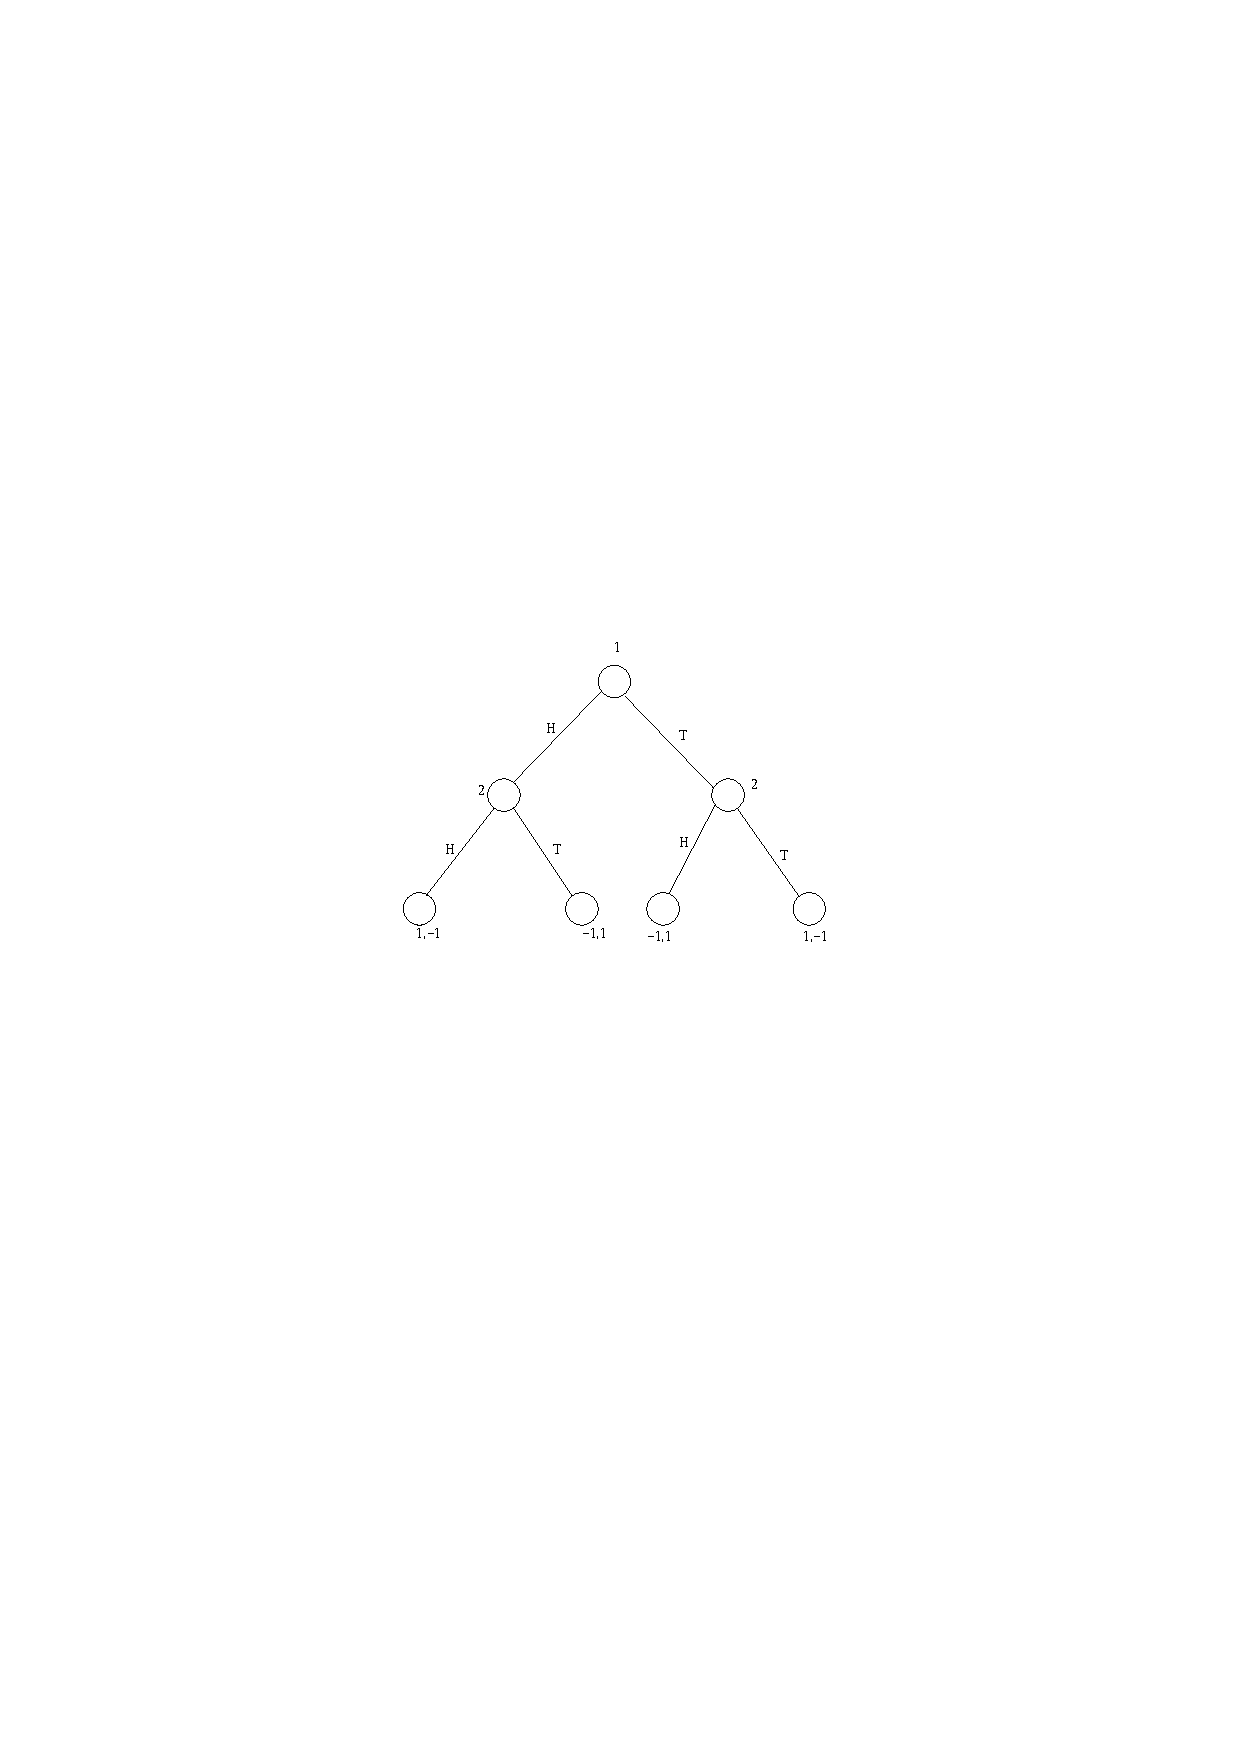
\includegraphics[width=\linewidth]{mpwo1.pdf}
		% 	\caption{Player 1 moves first}
		% 	\label{fig:mpwo1}
		% \end{subfigure}
		% \vLine
		% \begin{subfigure}{0.45\linewidth}
		% 	\centering
		% 	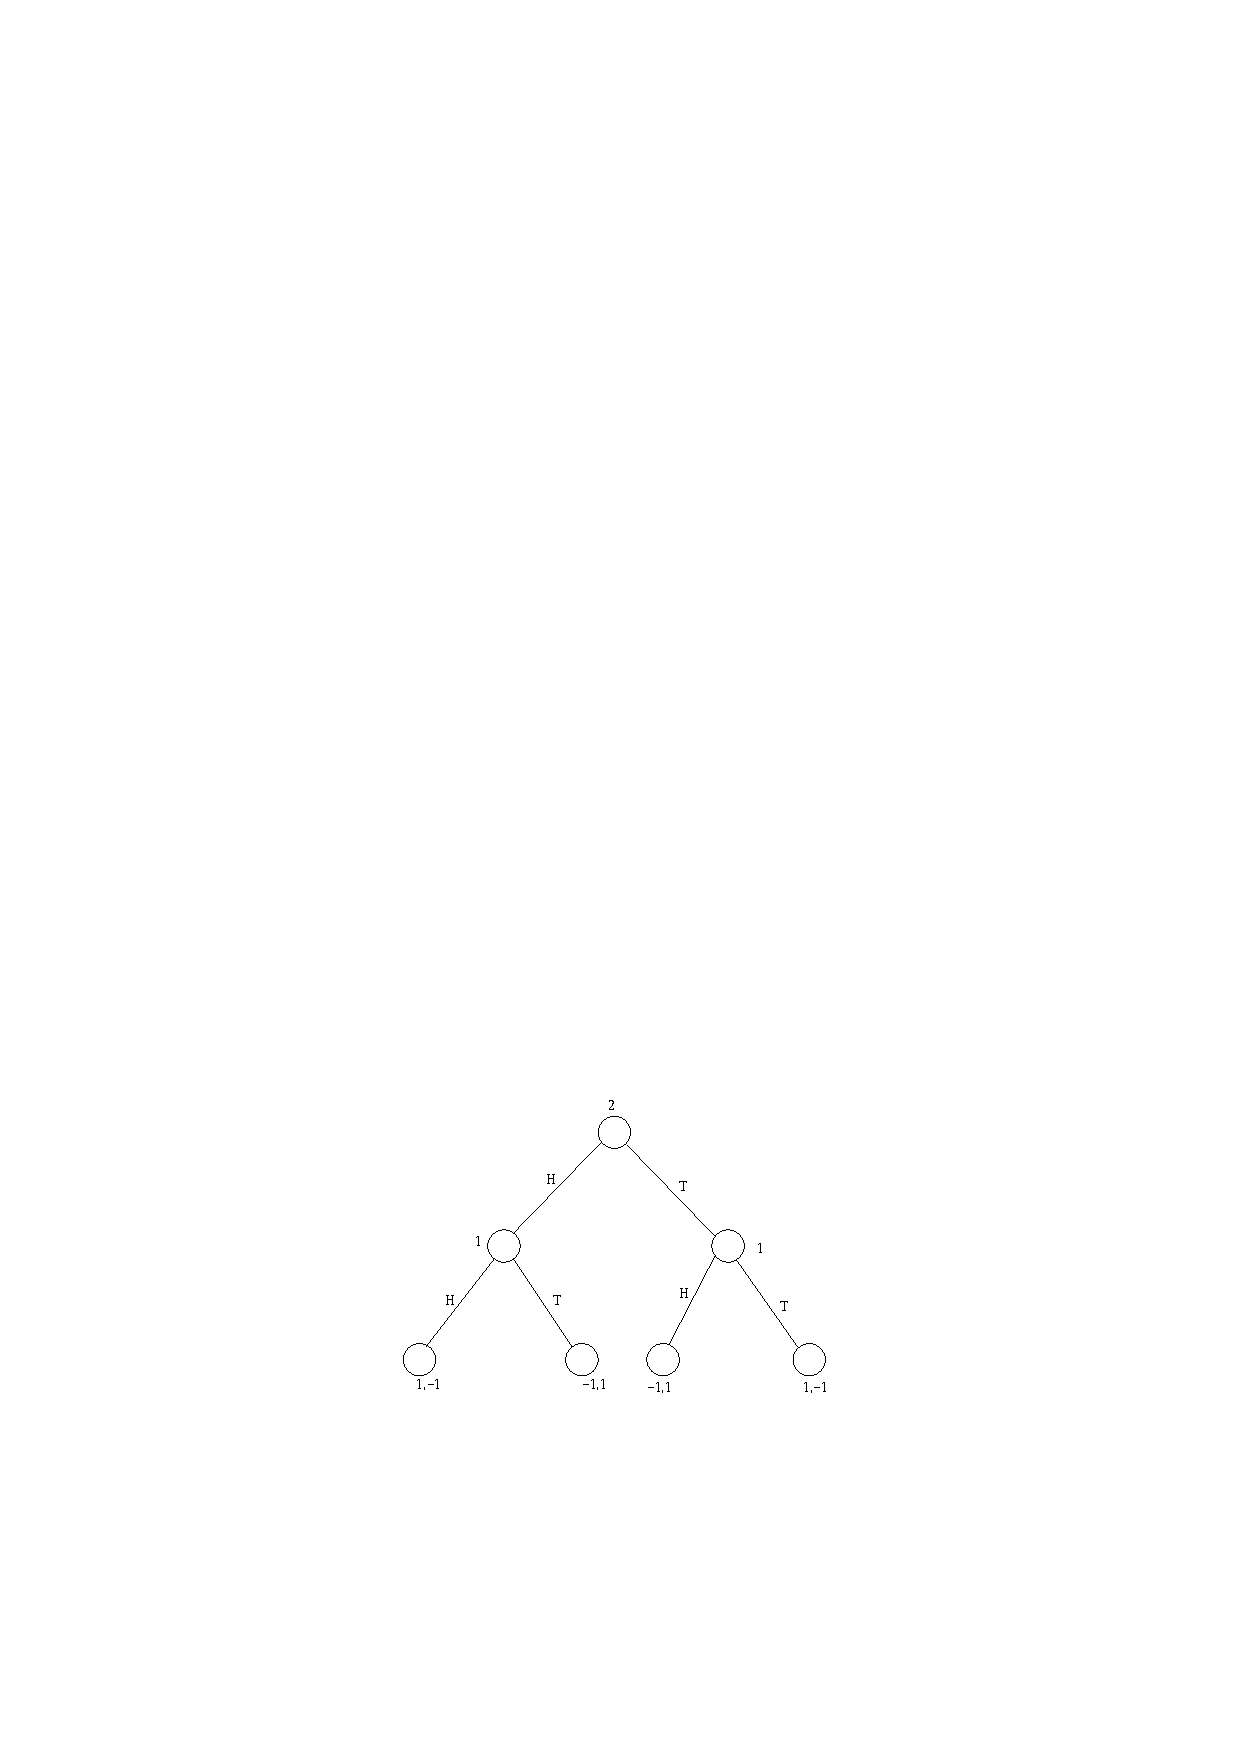
\includegraphics[width=\linewidth]{mpwo2.pdf}
		% 	\caption{Player 2 moves first}
		% 	\label{fig:mpwo2}
		% \end{subfigure}
		\caption{Matching pennies game with observation}
		\label{fig:mpwo}
	\end{figure}
	For this game in Figure \ref{fig:mpwo1}, we have
	\[N = \{1, 2\}\]
	\[A_1 = A_2	 = \{H, T\}\]
	\[\mathbb{H} = \{(H,H), (H, T), (T,H), (T, T)\}\]
	\[S_\mathbb{H} = \{\varepsilon,H, T\}\]
	\[P(\varepsilon) = 1; P(H) = 2;\quad P(T) = 2\]
	\[\mathbb{I}_1 = \{\{\varepsilon\}\};\quad \mathbb{I}_2 = \{\{H\}, \{T\}\}\]
	\[u_1(HH) = 1;\quad u_1(HT) = -1;\quad u_1(TH) = -1;\quad u_1(TT) = 1\]
	\[u_2(HH) = -1;\quad u_2(HT) = 1;\quad u_2(TH) = 1;\quad u_2(TT) = -1\]
	Strategies of player 1 are $s_{11}: {\varepsilon}\rightarrow H$ and $s_{12}: {\varepsilon}\rightarrow T$, similarly for player 2 

	$s_{21}: {H}\rightarrow H; {T}\rightarrow H$, $s_{22}: {H}\rightarrow H; {T}\rightarrow T$, $s_{23}: {H}\rightarrow T; {T}\rightarrow H$ and $s_{24}: {H}\rightarrow T; {T}\rightarrow T$
\end{exm}
\begin{table}[H]
    \centering
    \subfloat[With Observation]{
    \begin{tabular}{ |c|c|c|c|c| } 
        \hline
        1/2 & $s_{21}$ & $s_{22}$ & $s_{23}$ & $s_{24}$\\\hline
        $s_{11}$ & $1,-1$ & $1,-1$ & $-1,1$ & $-1,1$\\\hline
        $s_{12}$ & $-1,1$ & $1,-1$ & $-1,1$ & $1,-1$\\\hline
    \end{tabular}}
\vLine
    \subfloat[Without Observation]{
    \begin{tabular}{ |c|c|c| } 
        \hline
        1/2 & $s_{21}$ & $s_{22}$\\\hline
        $s_{11}$ & $1,-1$ & $-1,1$ \\\hline
        $s_{12}$ & $-1,1$ & $1,-1$\\\hline
    \end{tabular}}
    \caption{Payoff Matrix for Matching Pennies}
\end{table}
\begin{exm}[Matching Pennies without Observation]
	In this case, one of the players places his rupee coin heads up or tails up.
	The other player does not observe the outcome and only puts down her rupee coin heads up or tails up. This is equivalent to the two players put down their rupee coins simultaneously.
	Depending on whether player 1 or player 2 moves first, there are two versions of this game. Figure \ref{fig:mpwoo1} shows the game tree when player 1 moves first while Figure \ref{fig:mpwoo2} shows the game tree when player 2 moves first.
	\begin{figure}[h]
		\centering
		\begin{subfigure}{0.45\linewidth}
		        \centering
		        \begin{tikzpicture}[scale=0.12, every node/.style={scale=0.7}]
		            \tikzstyle{every node}+=[inner sep=0pt]
		                \draw [black] (0,30) circle (2.5);
		                \draw (0,30) node {$1$};
		                \draw [black] (-15,15) circle (2.5);
		                \draw (-15,15) node {$2$};
		                \draw [black] (15,15) circle (2.5);
		                \draw (15,15) node {$2$};;
		                \draw (-25,-1) node {$(1,-1)$};
		                \draw (-5,-1) node {$(-1,1)$};
		                \draw (5,-1) node {$(-1,1)$};
		                \draw (25,-1) node {$(1,-1)$};
		                \draw (-8.5,23.5) node [left] {$H$};
		                \draw (8.5,23.5) node [right] {$T$};
		                \draw (-22,8) node [left] {$H$};
		                \draw (-8,8) node [right] {$T$};
		                \draw (8,8) node [left] {$H$};
		                \draw (22,8) node [right] {$T$};
		                \path [linedash] (-12.5,15) -- (12.5,15);
		                \path [line] (-1.5,28) -- (-13,17.5);
		                \path [line] (1.5,28) -- (13,17.5);
		                \path [line] (-16.5,13) -- (-25,1);
		                \path [line] (-13.5,13) -- (-5,1);
		                \path [line] (13.5,13) -- (5,1);
		                \path [line] (16.5,13) -- (25,1);
		            \end{tikzpicture}
		            \caption{Player 1 moves first}
		            \label{fig:mpwoo1}
		    \end{subfigure}
		    \vLine
		    \begin{subfigure}{0.45\linewidth}
		        \centering
		        \begin{tikzpicture}[scale=0.12, every node/.style={scale=0.7}]
		            \tikzstyle{every node}+=[inner sep=0pt]
		                \draw [black] (0,30) circle (2.5);
		                \draw (0,30) node {$2$};
		                \draw [black] (-15,15) circle (2.5);
		                \draw (-15,15) node {$1$};
		                \draw [black] (15,15) circle (2.5);
		                \draw (15,15) node {$1$};;
		                \draw (-25,-1) node {$(1,-1)$};
		                \draw (-5,-1) node {$(-1,1)$};
		                \draw (5,-1) node {$(-1,1)$};
		                \draw (25,-1) node {$(1,-1)$};
		                \draw (-8.5,23.5) node [left] {$H$};
		                \draw (8.5,23.5) node [right] {$T$};
		                \draw (-22,8) node [left] {$H$};
		                \draw (-8,8) node [right] {$T$};
		                \draw (8,8) node [left] {$H$};
		                \draw (22,8) node [right] {$T$};
		                \path [linedash] (-12.5,15) -- (12.5,15);
		                \path [line] (-1.5,28) -- (-13,17.5);
		                \path [line] (1.5,28) -- (13,17.5);
		                \path [line] (-16.5,13) -- (-25,1);
		                \path [line] (-13.5,13) -- (-5,1);
		                \path [line] (13.5,13) -- (5,1);
		                \path [line] (16.5,13) -- (25,1);
		            \end{tikzpicture}
		            \caption{Player 2 moves first}
		            \label{fig:mpwoo2}
		    \end{subfigure}
		\caption{Matching pennies game without observation}
		\label{fig:mpwoo}
	\end{figure}
	% \begin{figure}[H]
	% 	\centering
	% 	\begin{subfigure}{0.45\linewidth}
	% 		\centering
	% 		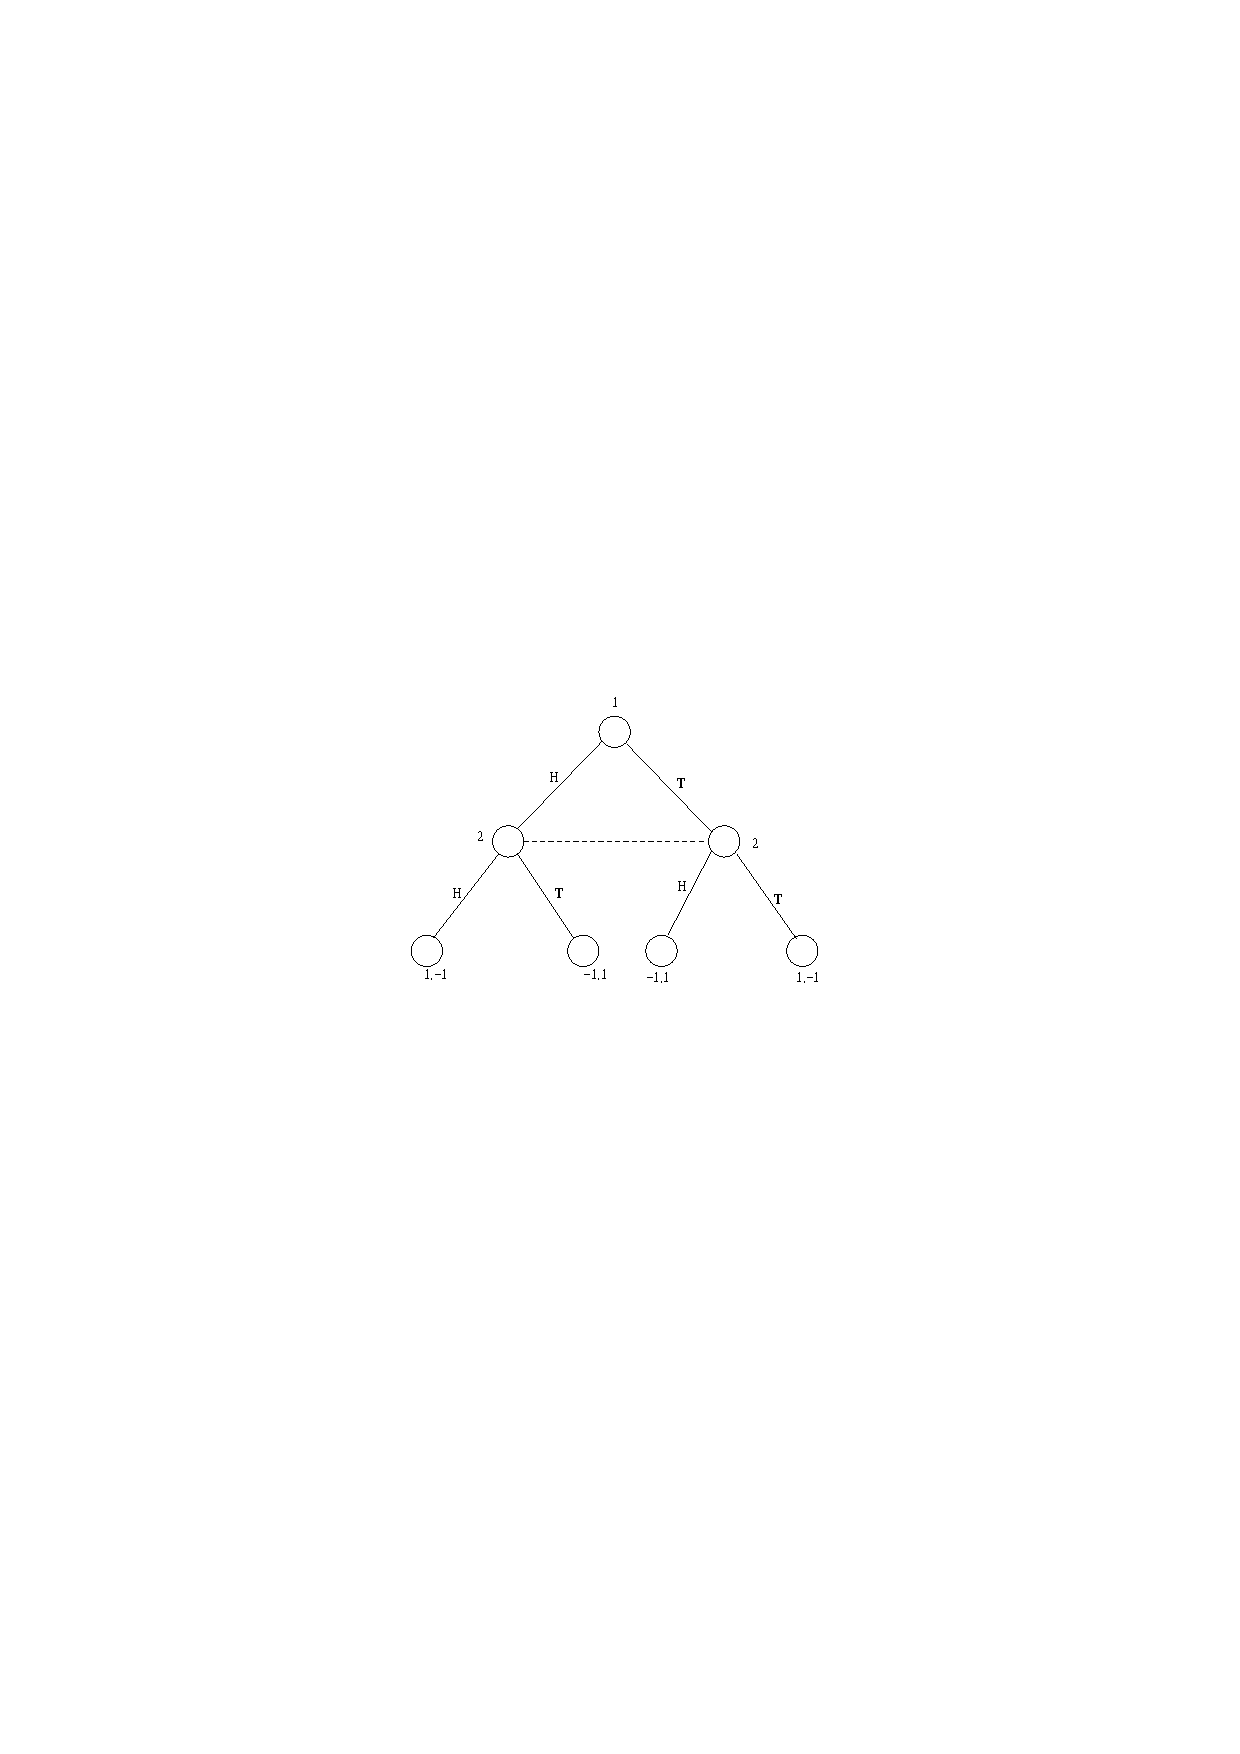
\includegraphics[width=\linewidth]{mpwoo1.pdf}
	% 		\caption{Player 1 moves first}
	% 		\label{fig:mpwoo1}
	% 	\end{subfigure}
	% 	\vLine
	% 	\begin{subfigure}{0.45\linewidth}
	% 		\centering
	% 		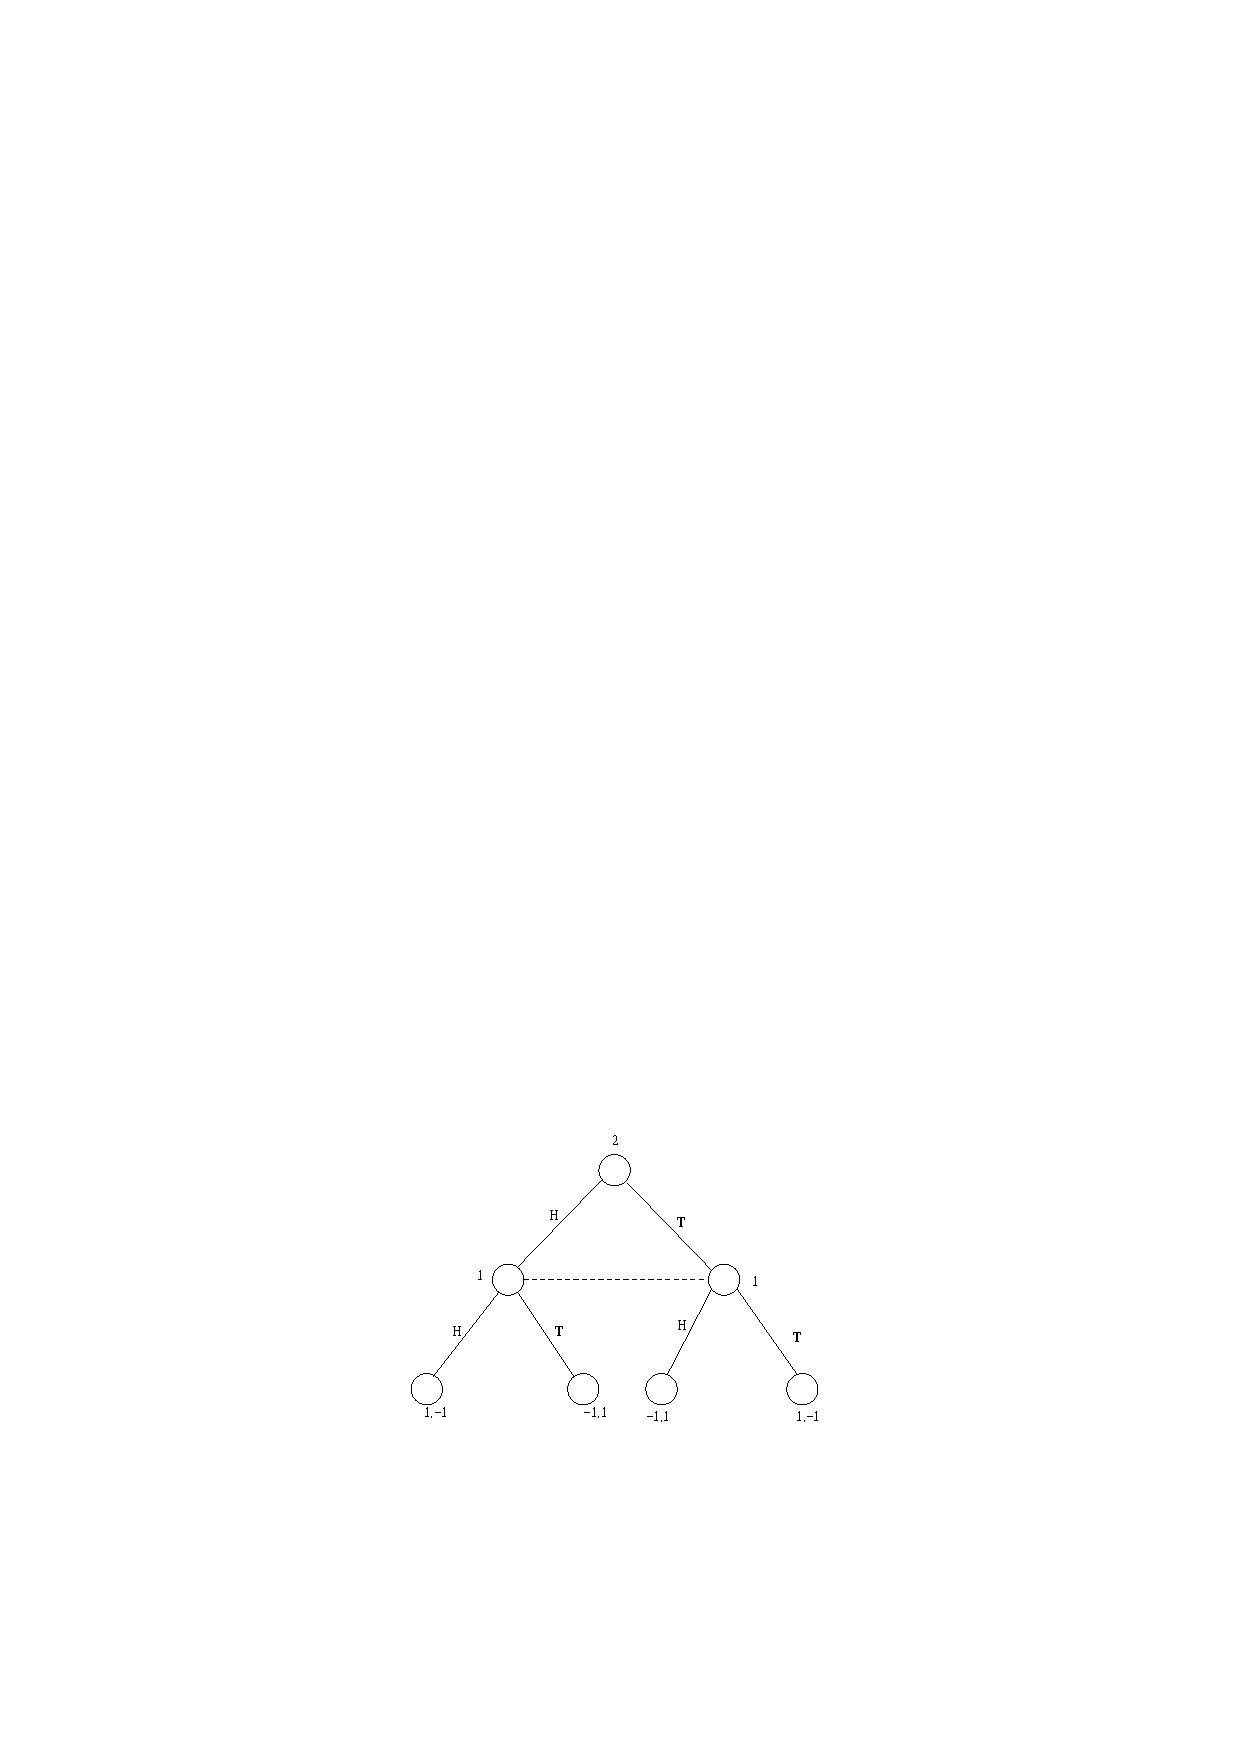
\includegraphics[width=\linewidth]{mpwoo2.pdf}
	% 		\caption{Player 2 moves first}
	% 		\label{fig:mpwoo2}
	% 	\end{subfigure}
	% 	\caption{Matching pennies game without observation when player 1 moves first}
	% 	\label{fig:mpwoo}
	% \end{figure}
	Note that the game trees of Figures \ref{fig:mpwo1} and \ref{fig:mpwoo1} are virtually the same except that the two decision nodes corresponding to player 2 in Figure \ref{fig:mpwoo1} are connected with dotted lines. Same case with Figures \ref{fig:mpwo2} and \ref{fig:mpwoo2}
	\begin{defn}[Information Set]
		An information set of a player is a set of that player's decision nodes that are indistinguishable to her.
		Since each decision node corresponds uniquely to a sequence of actions from the root node to the decision node, each information set of a player consists of all proper subhistories relevant to that player which are indistinguishable to that player. 
	\end{defn}
\end{exm}
\begin{note}
	Though the action sets of players can be deduced from terminal histories and the player function, we explicitly include action sets as a part of definition of an extensive form game for ease of understanding.
\end{note}
\begin{defn}[Perfect Information and Imperfect Information Games]
	An extensive form game with perfect information is one in which all the information sets are singletons.
	If at least one information set of at least one player has two or more elements, the game is said to be of imperfect information.
\end{defn}
In a game with perfect information, each player is able to observe all previous moves or the entire history thus far.
Each player knows precisely where she is currently and also knows precisely how she has reached that node.

Games in Figures \ref{fig:mpwo1} and \ref{fig:mpwo2} are games with perfect information while the games shown in Figures \ref{fig:mpwoo1} and \ref{fig:mpwoo2} are games with imperfect information.